\section{Small oscillations}\label{sec:3.5}
%\subsection{Aproximação para a órbita fechada e a compactação de momento}
We are now ready to analyse in detail the energy oscillations of the electrons in a bunch. I shall take up first the special case of the small (linearized) oscillations which occur so long as the variations of $\tau$ are limited to a small interval that corresponds to an approximately linear segment of $V(\tau)$. And then look later (in the following section) at the nonlinear oscillations which occur when the excursions of $\tau$ are large.

For small $\tau$ and $\epsilon$, we may replace $V(\tau)$ and $U_{rad}(\epsilon)$ by the linear approximations of Eqs. \eqref{eq:3.35} and \eqref{eq:3.23}. Then Eq. \eqref{eq:3.34} becomes
\begin{align}
	\frac{d\epsilon}{dt} = \frac{1}{T_0}(e\dot{V}_0 \tau - D\epsilon)\label{eq:3.40}
\end{align}
This equation can now be combined with Eq. \eqref{eq:3.32} to give a differential equation for $\epsilon$ or $\tau$. Suppose we choose $\tau$. Taking the time derivative of Eq. \eqref{eq:3.32} and eliminating $\epsilon$, you can show that
\begin{align}
	\frac{d^2 \tau}{dt^2} + 2\alpha_\epsilon \frac{d\tau}{dt} + \Omega^2 \tau = 0\label{eq:3.41}
\end{align}
with \footnote{Careful! There are not enough different letters. The constant $\alpha_\epsilon$ is a new quantity quite distinct from the dilation factor $\alpha$.}
\begin{align}
	\alpha_\epsilon &= \frac{D}{2 T_0}\\
	\Omega^2 &= \frac{\alpha\ e\ \dot{V}_0}{T_0\ E_0} \label{eq:3.43}
\end{align}

You will recognize that Eq. \eqref{eq:3.41} describes a damped harmonic oscillation with the oscillation (angular) frequency $\Omega$, and damping coefficient $\alpha_\epsilon$. Since the damping rate in a storage ring is always slow ($\alpha_\epsilon << \Omega$) the solution of Eq. \eqref{eq:3.41} can be written as
\begin{align} \label{eq:3.44}
	\tau(t) = A\ e^{-\alpha_\epsilon t} \cos(\Omega t - \theta_0)
\end{align}
with $A$ e $\theta_0$ arbitrary constants. Or, using the usual complex notation,
\begin{align}
	\tau(t) = \tilde{\tau}\ e^{-(\alpha_\epsilon - i\Omega)t}
\end{align}
where $\tilde{\tau}$ is a complex constant.

Equations \eqref{eq:3.40} and \eqref{eq:3.32} can be solved instead for $\epsilon$, which, you can show, satisfies the same differential equation as $\tau$, Eq. \eqref{eq:3.41}. And so the time variations of $\epsilon$ are
\begin{align}
	\epsilon(t) = \tilde{\epsilon}\ e^{-(\alpha_\epsilon - i\Omega)t}
\end{align}
From Eq. \eqref{eq:3.32} $\tilde{\epsilon}$ and $\tilde{\tau}$ are related by
\begin{align}
	\tilde{\epsilon} = -i\frac{\Omega E_0}{\alpha}\tilde{\tau}\label{eq:3.47}
\end{align}
(because $\alpha_\epsilon << \Omega$) and so the oscillations of $\epsilon$ and $\tau$ will have a phase difference of $\pi/2$.

Notice that the oscillation frequency of the small energy oscillations depends on the rf system only through $\dot{V}_0$. The frequency is proportional to the square root of the rf slope at the synchronous phase. The other parameters, $\alpha$, $T_0$, $E_0$ are characteristics of the guide field (including the energy at which it is operated). The damping constant of the energy oscillations $\alpha_\epsilon$ -- which is the inverse of the damping time constant - is proportional to $D$, which is the rate-of-change of the radiation loss with energy. As we shall see, this rate depends on the electron energy and on the properties of the guide field.

I would like to give now some orders of magnitude for the various quantities which have been appearing. The skeptical among you may then be happier about the approximations which have been made. A storage ring for 1 GeV electrons might have the following typical magnitudes for the various (angular) frequencies:
\begin{align*}
	\omega_r = 2\pi /T_0 &\approx 10^7 s^{-1}\\
	\omega_\beta = \nu \omega_r &\approx 3\omega_r\\
	\Omega &\approx 10^4 s^{-1}\\
	\alpha_\epsilon &\approx 10 s^{-1}
\end{align*}
The large ratios $\omega_r/\Omega$ and $\Omega/\alpha_\epsilon$ justify the approximations we have been making.

In the absence of damping $\epsilon$ and $\tau$ are conjugate variables. In a ``phase diagram'', where $\epsilon$ is plotted versus $\tau$, the oscillations are described by a point which moves cyclicly around an ellipse. See \autoref{fig:fig35}(a). The ratio of the two semimajor axes of the ellipse would be -- by Eq. \eqref{eq:3.47}
\begin{align}
	\frac{\epsilon_{max}}{\tau_{max}} = \frac{|\tilde{\epsilon}|}{|\tilde{\tau}|} = \frac{\Omega E_0}{\alpha}
\end{align}

\begin{figure}[!htb]
	\centering
	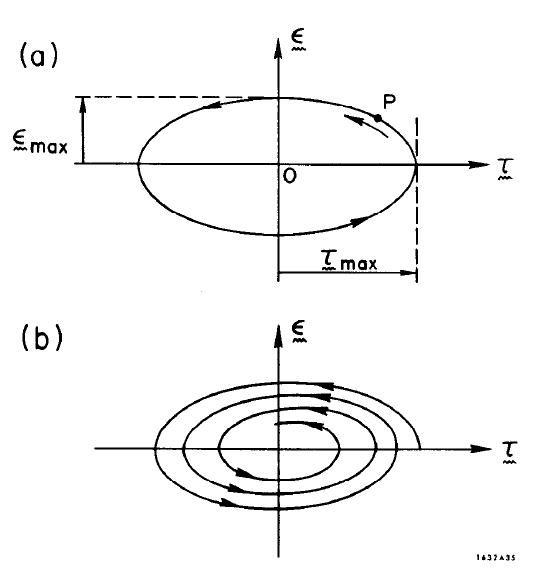
\includegraphics[width=0.6\linewidth]{./Figuras/fig35.jpeg}
	\caption{Phase diagram for energy oscillations. (a) Without damping. (b) With damping. (The damping rate is very much exaggerated).}
	\label{fig:fig35}
\end{figure}

If the scales are chosen so that the ellipse becomes a circle, the reference point rotates at the constant angular frequency $\Omega$. With damping, the size of the ellipse decreases slowly and the phase trajectory is a slow inward spiral as indicated crudely in \autoref{fig:fig35}(b). The phase diagram also makes transparent why the damping depends on $dU_{rad}/dE$. If this derivative is positive, the electron is losing a little extra amount of energy while on the upper half of the ellipse, and gaining a little extra energy while on the lower half. So it is always “drifting” toward the axis of $\tau$ and the oscillation amplitude is decreasing -- in proportion to $dU_{rad}/dE$.

According to our solution, the energy oscillations of all electrons should ultimately be completely damped out and they should all end up on top of the synchronous electron. But we have not yet taken into account the excitation of the oscillations by the quantum effects which “shake up” the oscillations and prevent them ever from going completely to zero. (They are considered in the next part). Under stationary conditions any stored electron will typically be found with some residual oscillation amplitude in which there is a balance between the excitation and the damping. Since both of these processes are slow we may think of the energy oscillation during any brief time as being described by a fixed phase ellipse such as the one in \autoref{fig:fig34}(a).

I should also remind you that the energy oscillations relate not only to the longitudinal oscillations (in $z$ or $\tau$) of the electrons in a bunch but have also a lateral component. According to Eq. \eqref{eq:3.3} an energy deviation $\epsilon$ results in a radical displacement $x_\epsilon$ which is proportional to $\epsilon$ and in phase with it. So the component $x_\epsilon$ of the total horizontal displacement oscillates in synchronism with the energy oscillations. Generally, this transverse manifestation of the energy oscillations has (under stationary conditions) about the same amplitude as the betatron oscillations.
